\chapter{Related Work}
\label{cha:related-work}


This chapter defines the previous work related to the project and defines and describes the technologies and frameworks used within the project. While the project is built based on the technologies discussed within the scope of the course, the inspiration has been found while reviewing literature on applications of IoT technology specifically [ref Smart office energy management system using bluetooth low energy based beacons and a mobile app]. This has shown that simple BLE Beacons and mobile application can be used within building automation environment. Further experiments have been made in order to determine potential of wireless sensor networks and bluetooth technology to monitor refridgerated containers during transport[ref Review. Monitoring the intermodal, refrigerated transport of fruit using sensor networks] and have concluded that while the technology is available, it is primarily the lack of standardization of technologies within IoT enironments and transport systems (where CAN Bus is prevalent) that slows down adoption of WSN technology for monitoring of containers. Due to the lack of standardization several competing radio technologies in the arena of wireless sensor networks have been discussed as well such as 802.15.4 and its usage within (among others) Zigbee technology. Bluetooth low energy has however advantage in its integration to most of the modern smartphones and the growth potential of the technology [ref https://www.statista.com/statistics/750569/worldwide-bluetooth-low-energy-device-market-volume/]. Its ready availability was a determining factor in choosing the technology for status broadcasting within this project. It is also expectable that the application will focus on more advanced use cases due to possibility of creation of a 6LoWPAN[ref] network over BLE system. 

\bigskip

It would be unfair not to mention a very comprehensive book [ref Beginning Sensor Networks with Arduino and Raspberry Pi] on starting with wireless sensor networks and their applications. While the book does primarily consider Zigbee for networking the inspiration for building monitoring systems with data storage has had effect on the ideas behind the project. The project also considered on how to create a SCADA system (in our case very simple) for IoT based environment and mobile users. This have provided an interesting topic as the SCADA system of the future will have to be able to handle IoT environments, specifically the data loads and connectivity. Proposed architectures and frameworks are starting to emerge [ref An IoT architecture for things from industrial environment]. Often a research focus is within terms of security of these system [ref Cloud-Assisted IoT-Based SCADA Systems Security: A Review of the State of the Art and Future Challenges], which we have not considered within our implementation, however provided us with several thinking points on how such system will have to look if it was to be ever deployed within the maritime industry (or container shipping industry in general).

\bigskip

It is equally important to mention that it was the development of mobile operating systems such as Google Android [ref] and its rich APIs, which enabled us easy programmatic access to Bluetooth radio within the phone as well as communication within the IoT device itself.


\section{Frameworks and Technologies}
\label{sec:fram-techn}

As many IoT based environments, the container monitoring system is comprised of multitude of frameworks, devices, communication paradigms and programming languages.

\subsection{Node.js}
\label{subsec:Node}

Often know as the javascript for the server side it is javascript runtime built on the Chrome's V8 javascript engine. The development in Node.js typically confirms with principles of event driven applications with non blocking I/O [ref]. Primary purpose of Node.js is to provide environment for building of scalable network applications. This is done by usage of asynchronous processing, where connections to the server fire a callback that further handles the processing of the request and provides a reply to the client. Very common usage of Node.js is in development of REST based web APIs (more about REST is here \autoref{subsec:rest}).

\bigskip
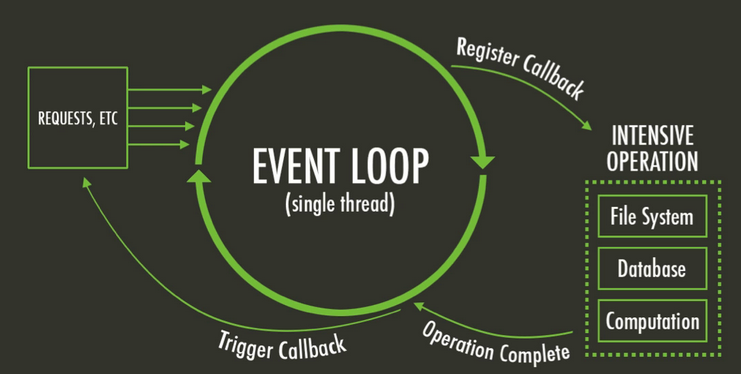
\includegraphics[scale=0.3]{gfx/node} 
\bigskip

Node.js has been used within the scope of our project to develop the central server and the client on Raspberry PI(what we consider a BLE beacon device). Node.js consists of multitude of frameworks and we have primarily used Express framework for web application development and Sequelize ORM for database connectivity. The package manager used was the Node.js native package manager npm [ref], which is one of the most widely used package managers within javascript development.

\subsubsection{Express framework}
\label{subsubsec:express}

Express framework is a minimalistic web framework for Node.js[ref]. It simplifies the development of web applications and web APIs. Express is not only used to develop web applications but is often used to create other frameworks with notable examples of Sails which is an MVC framework for web application development and LoopBack, which is used to develop end to end REST APIs. The way of creating a REST method in express is simple and goes as (example of simple GET method):\newline 

\smallskip
{\textbf app.get('/', (req, res) => res.send('Hello World!'))}
\newline
\smallskip

The simplicity of use and sufficient community of users have been the primary drivers behind using Express for development of web features (Primarily REST APIs, but also HTTP server initialization) within our system.

\subsubsection{Sequelize ORM}
\label{subsubsec:sequelize}

To (use an) ORM or not to (use an) ORM... This is a question that is often pondered when starting a new project, which requires relational database as a persistant data storage. Our decision to use the ORM was primarily based on the wish to learn about ORM within the Node.js environment. Sequelize is one of the prominent ORMs within the Node.js ecosystem [ref]. It is promise based, hence all of the operations are handled asynchronously. The ORM has bindings to PostgreSQL, MySQL, MariaDB, SQLite and Microsoft SQL Server. Current versions of sequelize supports Node.js version 4 or above. Sequelize lends itself well for implementation of the repository pattern as it allows for simple definitions of database entity models, database operations on these models as well as definitions of relationships between them. Also datatypes are present for mapping of database supported datatypes to datatypes supported by Node.js. Sequelize is a so called "leaky ORM" meaning that it enables of passing of raw SQL statements to be executed in order to support cases where entity model based querying would be too complex to use. An example of an entity model in sequelize (all of the database tables within our project have entity models created):\newline

\smallskip
\begin{lstlisting}
    var Users = sequelize.define('USERS', {
            Id: {type: DataTypes.INTEGER, primaryKey: true, autoincrement: true},
            Name: {type: DataTypes.STRING},
            Function: {type: DataTypes.STRING}
        },
        {
            freezeTableName: true,
            tableName: 'USERS',
            timestamps: false
        });
\end{lstlisting}
\smallskip

\subsubsection{Bleno}
\label{subsubsec:bleno}

Bleno is a Node.js module used to implement BLE peripherals [ref]. Bleno can be used to enable the advertising mode (as used within our project) or to facilitate simple (peripheral to central) data transfers via BLE (BLE technology is described here \autoref{subsec:bluetooth}). Bleno is available in NPM and hence fits perfectly to the Node.js development pipeline. Bleno provides simple way of advertising (broadcasting) data: \newline

\smallskip
{\textbf bleno.startAdvertising(name, serviceUuids[, callback(error)]);}
\newline
\smallskip

\subsection{Android (Java)}
\label{subsec:android}
It is thanks to the development of mobile operating systems and SDKs that it has been possible to create the project in such a short time. The Android mobile operating system [ref] does not need introductions. It is the most widely used mobile operating system in the world that exposes rich Java based APIs that enable rapid application development and easy access to the communication subsystem (in our case BLE) within the mobile device. The operating system supports wide variety of devices and chipsets.


\subsection{Bluetooth Low Energy}
\label{subsec:bluetooth}
Bluetooth Low Energy is the technology introduced by the Bluetooth Special Interest Group [ref] in order to create low energy version of Bluetooth suitable for IoT environments. This comes at the cost of loss of compatibility with the Bluetooth Classic protocol. Todays low cost computing devices (for example Raspberry PI) often include BLE and hence make the technology ubiquitous. BLE has been primarily designed for short data bursts status communication where devices would communicate some measured phenomena on a periodic basis. It has also introduced a so called broadcast (advertising) mode where the device can act as a beacon advertising some predetermined information. The information advertised can be static, as is often the case of BLE beacons [ref] or dynamic as is a case within our project. 

\bigskip

In order to stay within the energy consumption envelope this of course has limitations. The advertising mode can at maximum transport 31 Bytes of data payload. Advertisement mode broadcast the data and any Bluetooth Low Energy device in the vicinity can pick up the data payload advertised. The package structure of the BLE Advertisement package:

\bigskip
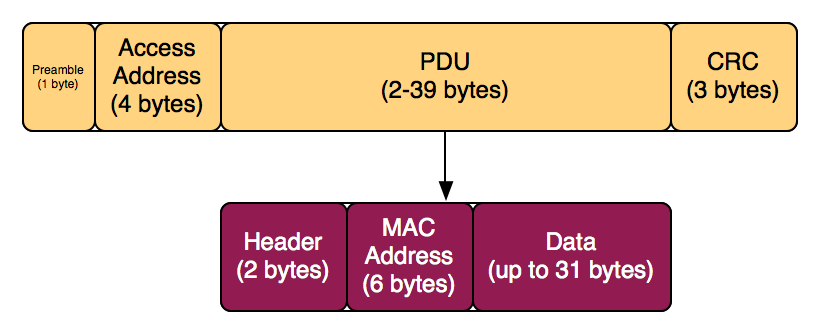
\includegraphics[scale=0.4]{gfx/blepacket} 
\bigskip  

\subsection{SQLite}
\label{subsec:sqlite}
SQLite is a library providing a serverless, transctional and self contained SQL database engine [ref]. The embedded database engine provided by SQLite is cross platform and simply deployable by usage of a NPM package. Since the SQLite is part of a public domain, it is simple to use without any license considerations. While the datbase engine itself is considered lightweight, the maximum database size is approximately 140TB. This is more than sufficient for the needs of the project. SQLite has support for most of the standard SQL features, while the unsopported features were not a concern to us. Currently SQLite can be found on devices ranging from servers to embedded computers.

\subsection{RESTful communication}
\label{subsec:rest}
Representational state transfer (REST) provides a way of communicating between devices using Web resources. The base for the communication is HTTP protocol (but not only, COAP would be a nice example of a REST protocol for constrained devices) which implements methods that describe the action (GET, POST, PUT, DELETE, etc.) to be udertaken on the particular web resource. The data can be exchanged between these endpoints in variety of forms (JSON, XML, HTML, etc.). The course book [ref] has a definition of REST that was considered within this project. The statelessness of the RESTful communication as well as unique identification of resources by usage of URIs is what makes it a good fit for data exchange within the Web of Things. REST is currently a popular way of defining Web APIs and many programming languages provide (at least one) framework specifically oriented at creation of REST Web APIs. The example REST call looks as follows:

\bigskip
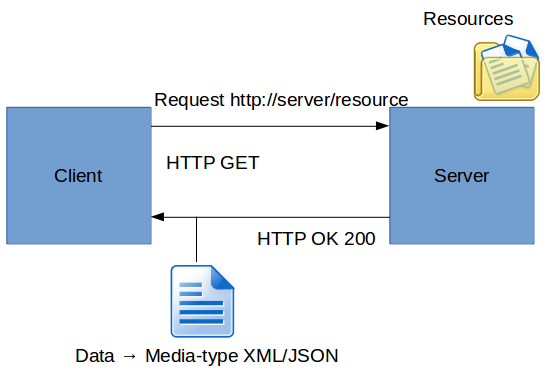
\includegraphics[scale=0.5]{gfx/REST} 
\bigskip

\subsection{WebSocket}
\label{subsec:websocket}
WebSocket is a communication protocol that provides bidirectional communication over a single TCP connection [ref]. WebSockets primary functionality was to provide interaction between the client and the server with less overhead than long polling practices. The WebSocket is a part of the HTML5 specification. Due to the handshake implemented by WebSocket protocol (HTTP compatible) it can traverse proxy servers if the client is behind these. The WebSocket delivers live updates to the browser without the need of a page reload. Most of the modern Web browsers support the WebSocket protocol [ref].

%%% Local Variables:
%%% mode: latex
%%% TeX-master: "../ClassicThesis"
%%% End:
